\documentclass{spie}

\usepackage{amsmath}
\usepackage{amssymb}
\usepackage{fontawesome}
\usepackage{graphicx}
\usepackage{hyperref}
%\usepackage{mhchem}
\usepackage{siunitx}
\usepackage{units}

\pdfmapfile{=fontawesome.map}

\title{A cryogenic testbed for the characterisation of large detector arrays for astronomical and Earth-observing applications in the near to very-long-wavelength infrared}

\author[1]{Thomas L. R. Brien}
\author[1]{Peter A. R. Ade}
\author[2]{Markus Haiml}
\author[1]{Peter C. Hargrave}
\author[2]{Holger H\"ohnemann}
\author[1]{Enzo Pascale}
\author[1]{Rashmi V. Sudiwala}
\author[3]{Dirk Van Aken}

\affil[1]{School of Physics and Astronomy, Cardiff University, The Parade, Cardiff, CF24 3AA, UK}
\affil[2]{AIM Infrarot-Module GmbH, Theresienstra{\ss}e 2, D-74072 Heilbronn, Germany}
\affil[3]{Caeleste CVBA, Hendrik Consciencestraat 1B, B2800 Mechelen, Belgium}


\authorinfo{Corresponding author: T. L. R. Brien (\faicon{envelope-o} \href{mailto:tom.brien@astro.cf.ac.uk}{tom.brien@astro.cf.ac.uk})}

\begin{document}
\maketitle

\begin{abstract}
In this paper we describe a cryogenic testbed designed to offer complete characterisation---via a minimal number of experimental configurations--- of mercury cadmium telluride (MCT) detector arrays for low-photon background applications, including exoplanet science and solar system exploration. Specifically, the testbed offers a platform to measure the dark current of detector arrays at various temperatures, whilst also characterising their optical response in numerous spectral bands. The average modulation transfer function (MTF) can be found in both dimensions of the array along with the overall quantum efficiency. Working from a liquid-helium bath allows for measurement of arrays from $4.2~\si{\kelvin}$ and active-temperature control of the surface to which the array is mounted allows for characterisation of arrays at temperatures up to $80~\si{\kelvin}$, with the temperature of the array holder known to an accuracy of at least $1~\si{\milli\kelvin}$, with the same level of long-term stability.
\end{abstract}

\keywords{Mercury cadmium telluride, MCT, low-temperature array characterisation}

\section{Introduction}
In recent years there has been a significant rise in the number of confirmed exoplanets discovered, indeed at time of writing there are over three thousand confirmed exoplanets with a further 4,600 candidate planets found by the \textit{Kepler} observatory \cite{NASAexoplanet} and ESA's \textit{Gaia} mission expected to find tens of thousands more \cite{Perryman2014}. However, the study of these objects has, so far, been predominately limited to determining their size, mass and orbital characteristics. The chemistry of exoplanets is a key area which must be explored in order to gain a more complete understanding of these astronomical objects, including knowledge of the constituent elements within their atmosphere, along with the nature of the planet's formation.
\par 
Such a study of exoplanet chemistry requires high-quality spectroscopy from the the visible to mid- and long-wave-infrared wavelength, with a spectral resolving power, $\mathcal{R} = \nicefrac{\Delta\lambda}{\lambda}$, of $\mathcal{R} \sim 100\mbox{--}300$ for most molecular signatures. Some species however require a much higher resolving power. \cite{Tinetti2013} To achieve such high-quality spectroscopy the currently favoured approach is to use a grating- or prism-based spectrograph combined with a high-resolution (high pixel count) photovoltaic array, typically a mercury cadmium telluride (MCT) array\cite{Glauser2013,Tinetti2015}. In this configuration, the image at the detector array contains the spectral information in one axis and spatial information in the perpendicular axis. The spectral resolution, $\Delta\lambda$, is limited by the dimensions of the collimated bin on the dispersive element and the pixel pitch of the array, along with the electro-optical characteristics of the array (such as cross-talk between pixels).
\par 
The study of exoplanets involves measuring relatively small dips in the light curve of an exoplanet-star system. These dips occur both when the planet transits the star, blocking light from the star; and when the exoplanet is eclipsed by the star, meaning light from only the star (as opposed to star $+$ planet) is received---clearly this situation is much less pronounced than the former. The variations in flux can be even fainter when one wishes to inspect the spectral properties of a light curve, as opposed to simply the total flux. The dark current limits the minimum detectable signal by reducing the achievable signal-to-noise ratio (SNR) for a given integration time. There is currently a lack European-manufactured detectors capable of operating a sufficiently low dark current for the next generation of observatories for exoplanet science. This has resulted in the European Space Agency (ESA) funding a program of work to support the European development of low dark current long- and very-long-wave infrared detectors.\footnote{See acknowledgements for ESA program number} In this paper we present a cryogenic testbed designed to offer flexible characterisation of the next generation of MCT detectors and also describe what tests---in addition to measurements of the dark current---are needed in order to determine the suitability of particular MCT arrays for use in astronomical and Earth-observing applications.
\par 
The initial configuration of the testbed discussed here is such that it can be used to ascertain two of the key performance parameters of MCT detectors, namely their dark current and cut-off wavelength. While this means that the initial spectral bands are beyond those of currently proposed exoplanet observatories\cite{Tinetti2015} or those studying high-redshift objects\cite{Flare2016}, bands more appropriate for these instruments may be studied by simply replacing pass-band filters. Indeed, while low-background applications, such as exoplanet transit spectroscopy, are considered here due to their challenging requirements on detector technologies, the testbed described may, through minor changes to its configuration, be used to characterise arrays for many applications; including those under high background such as Earth observing or the study of objects within our solar system; where photovoltaic detectors, such as MCTs, are commonly used.\cite{Donlon2012,Sonnabend2008}
\par 
We note that throughout this paper the term \textit{array} is taken to refer to a final hybrid detector package consisting of the array of photovoltaic pixels and any readout integrated circuit (ROIC) but does not include any further readout circuitry, such as any application-specific integrated circuit (ASIC).

\section{Key array quantities for characterisation}
In order to design a testbed capable of ascertaining the suitability of a particular array for low-background astronomical applications (such as exoplanet transit spectroscopy), it is important to first assess which parameters need to be studied and what impact reduced performance in a particular area would have on the instrument design and its performance. We have identified the following quantities as those most in need of measurement:
\begin{description}
\item \textbf{Dark current} At present the dark current is one of the major performance-limiting factors in the use of MCT detectors for astronomical observations. The dark current is manifested as an integrating signal during the readout of a photovoltaic array and has the effect of limiting the achievable signal-to-noise ratio from the ideal (photon-noise-limited) case.
\item \textbf{Spectral response} The key spectral parameter is the wavelength at which the array ceases to respond to an optical signal (this is related to the band gap of the material used). Furthermore, the detection efficiency through the spectral band of interest is important for understanding the uniformity of the spectral response.
\item \textbf{Operation temperature} While, in deployment, the detector array would be operated at a constant temperature, it is important to understand the behaviour of the array through the possible operational temperature range (nominally $20\mbox{--}80~\si{\kelvin}$) such that performance vs thermal budget can be assessed. This is of particular significance for application in Earth observing.
\item \textbf{Optical properties} Several optical characteristics are key to the suitability of an array for the applications under consideration here. Of particular interest is the image lag (see Section~\ref{sec:lag} for a discussion of the appropriate measurement of image lag for an astronomical instrument). The modulation transfer function (MTF, the ability to reproduce a spatially varying signal as a function of spatial frequency) also requires exploration.
\item \textbf{Electrical properties} The electrical properties of interest are, for the most part, those common to most detector arrays and include: noise of all types based both in the photovoltaic pixels as well as the readout, response non-uniformity, pixel-to-pixel cross talk, along with standard current-voltage ($I\mbox{-}V$) curves.
\end{description}
%
\section{Appropriately quantifying image lag for astronomical applications}\label{sec:lag}
Image lag is the fractional amount of an image recorded in one frame that exists in the subsequent frame. It is often thought of as a \textit{memory}, \textit{persistence} or \textit{ghosting} effect and is commonly measured by examining the remaining signal after an array is taken from an illuminated state in one frame to a blanked (dark) state in the following. We argue that, when considering astronomical applications, the reverse case whereby an array is taken from darkness in one frame to an illuminated state in the subsequent, is worthy of exploration. The reasoning for this can be understood by noting that this situation is the same as opening the shutter of a telescope and observing a source. Berta et al. (2012)\cite{Berta2012} show observations of the exoplanet GJ1214b using the \textit{Hubble} Space Telescope. They show that for each group of measurements, from the start of an exposure, the measured signal increases until a steady state is reached. This is attributed to ``charge trapping'' within the detector array. This trapping of charges results in some fraction of the charges generated by photons within the photovoltaic pixels not reaching the readout in the timescale of a single frame (or indeed the subsequent frames presented by Berta et al.). The ramps observed by Berta et al. (which were well documented for the WFC3 instrument on board \textit{Hubble}) are explained by the difference between the number of charges generated (charges in) and that reaching the readout (charges out). The ramp increases until all the charges generated in the first frames after opening the instrument's shutter have all reached the readout, after this there is a equilibrium between the consistent rate of charge generation (assuming the source brightness is constant) and the rate at which \textit{trapped} charges are released.
%\begin{figure}[tb]
%\begin{center}
%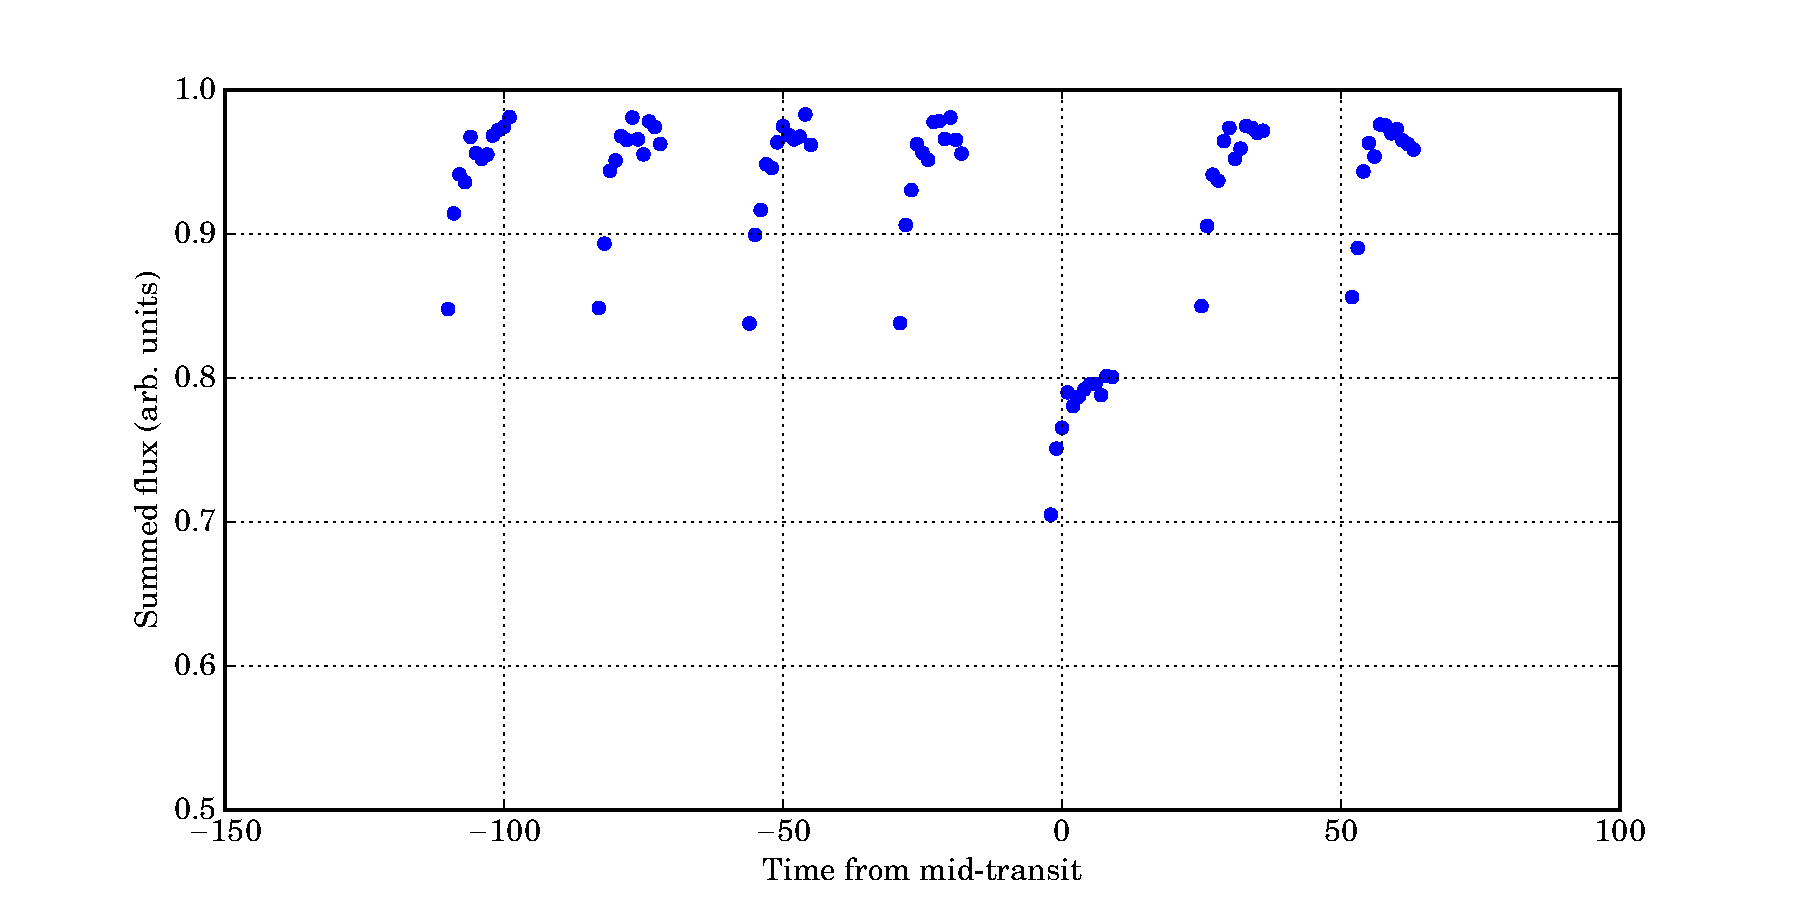
\includegraphics[height=0.35\textheight]{24_MCT_imageLagEx}
%\caption{Example of the persistence phenomenon as observed by Berta et al. using WFC3 on \textit{Hubble}. The data are divided into sets of twelve points after which the shutter is closed and data is downloaded from WFC3's buffer. The fifth set of data points corresponds to the point where a target planet is transiting its host star and thus blocking some light from the star. Based on Berta et al. (2012).\cite{Berta2012}}
%\label{fig:imageLag}
%\end{center}
%\end{figure}
\par 
This phenomenon is illustrated in Figure~3 of Berta et al.\cite{Berta2012} The data are divided into sets of twelve data points with each data point corresponding to the summed flux over some integration time. Between each set of points there is a blanked time while data are downloaded from WFC3's buffer. During this time the instrument's shutter is closed. It is clear that for each set of summed fluxes the initial values appears to be lower than the steady state reached before the buffer download. It is also clear that this is repeatable and dependant upon the illumination received. This can be seen in the third set of observations in the upper segment of Berta et al. Figure 3, which correspond to the point where the target planet is in front of its parent star and thus partially blocking the light from the star.
%
\section{Testbed design}\label{sec:design}
\subsection{Overall System Layout}\label{ssec:layout}
\begin{figure}[htb]
\begin{center}
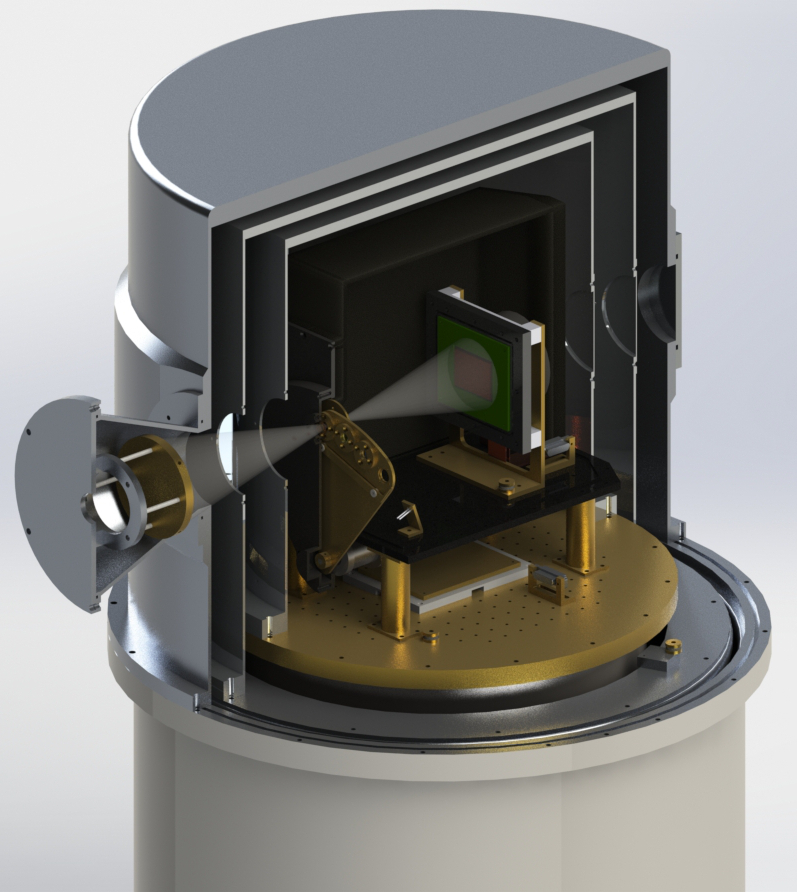
\includegraphics[height=0.5\textheight]{MCT_cryostat_ISO}
\caption{Rendered CAD model of testbed. The MCT array (shown in red for clarity) observes a black-body source through a set of infrared filters and a pinhole aperture. The filters are mounted to a segment of a filter wheel whose position is controlled by a cryogenic-certified stepper motor. The array is mounted via an L-bracket to an elevated optical bench and surrounded by a shield made from aluminium and anodised black to reduce reflections. Both are in excellent thermal contact with the 4.2-Kelvin plate of the liquid-helium cryostat; the array is thermally isolated via fibreglass (G-10 CR) standoffs. The observed beam is illustrated and it can be seen that the array is over illuminated below the vignetting limit.}\label{fig:cryostatISO}
\end{center}
\end{figure}
The testbed is designed around a Janis Research liquid-helium cryostat and is illustrated in Figure~\ref{fig:cryostatISO}. The detector array is mounted from a L-shaped bracket on an elevated optical bench (EOB) such that it is aligned with the optical axis of the cryostat. The detector array itself is mounted to a base plate made from a thermal conductive material which offers excellent matching to the coefficient of thermal expansion (CTE) of the array. The elevated optical bench is made from aluminium and is coated with a black pigment through anodising, this reduces the intensity of reflections to better than 5~\%; at interfaces between components (such as the detector bracket) the anodised finish is removed to improve thermal conduction. A shield structure is mounted from the EOB and contains a light-tight, double-lip interface to the EOB itself. The optical power on the array is defined by a pin-hole aperture in the EOB's shield. This aperture may be replaced by other apertures to vary the systems throughput or removed all together and replaced with a blank to achieve the darkest-possible configuration.\footnote{The base plate has the facility for a light-tight cap to be installed over the array; this means that the array does not observe the EOB's shield. We do not, however, consider this the darkest case possible since the cap will be at the temperature of the array carrier (up to $80~\si{\kelvin}$) whereas the OEB shield is at the lower temperature of $4.2~\si{\kelvin}$ and thus results in a lower photon flux on the array. The cap does however provide convenient protection for the array both during transit and when in storage.}
\par 
Beyond the EOB shield (along the optical axis) is a filter wheel (reduced to a fan shape for reasons of space), this contains three long-wave-infrared filters along with one open position and numerous blanked positions (the spaces between and beyond the filters), and is used to select the spectral band. The filter wheel is positioned by a cryogenically-certified stepper motor which has a step size of $0.037\si{\degree}$ ($9800~\mathrm{steps/rev.}$). Absolute positioning of the filter wheel is achieved through step counting and the use of limit switches. While the motor's cryogenic design should ensure that no steps are skipped---something we have supported through preliminary component testing---we note that the radial size of the beam at the filter wheel is $\sim 1.5~\si{\milli\metre}$ whereas the clear aperture radius for each filter is $4~\si{\milli\metre}$, allowing for an inaccuracy of $\pm 2.5~\si{\milli\metre}$ in position without cutting the beam. The distance from the centre of each filter to the motor shaft is $177.5~\si{\milli\metre}$ so the acceptable angular error is $\pm 0.8\si{\degree}$, which corresponds to $\pm 21$ steps of the motor. Stray light routes around the filter wheel are removed by a baffling structure which surrounds the filter wheel.
\par 
A temperature-controllable stage, located beneath the EOB, offers a mounting location for interface electronics and signal conditioning.
%
\subsection{Optical Design and Black-Body Source}\label{ssec:opticalDesign}
The optical configuration of the testbed is relatively simple. Spectral bands are defined by selecting a bandpass filter via the filter wheel, with each bandpass having a width of close to $10~\%$ its peak frequency. A short-wave-pass (SWP) filter removes any higher-wavelength leaks. In the initial test configuration there will be three spectral bands centred around $8$, $10$, $12~\si{\micro\metre}$, along with an \textit{open} position limited only by the SWP filter. The transmission of these filters has been measured at $77~\si{\kelvin}$ and is illustrated in Figure~\ref{fig:filters}. Prior to array testing, the filters will be remeasured at $4.2~\si{\kelvin}$ and the SWP measured to shorter wavelengths. Since the spectral band is simply defined by a pair of filters, it is trivial to reconfigure the testbed to characterise arrays at other wavelengths and for other applications, indeed the overall optical design of the testbed could be used for measurements from the optical to towards the far-infrared.
\begin{figure}[htb]
\begin{center}
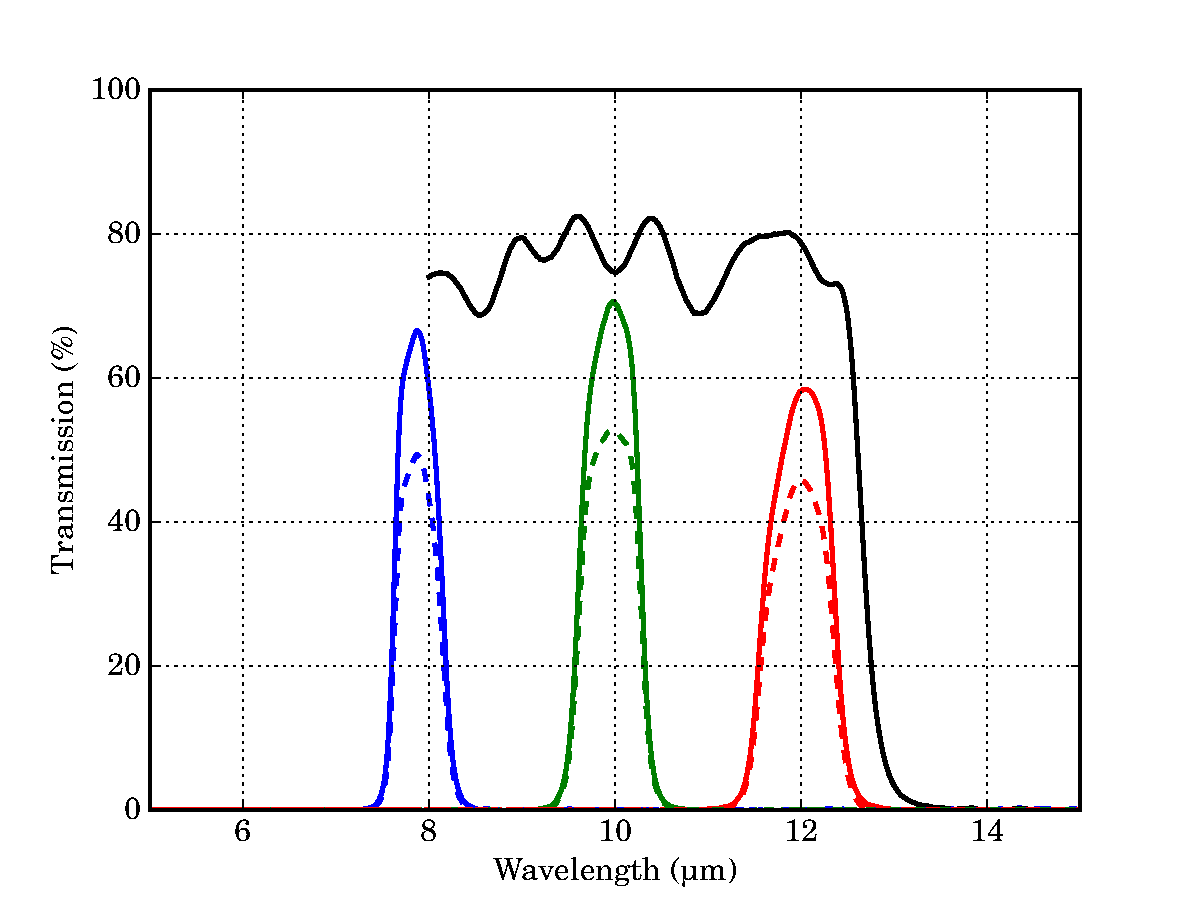
\includegraphics[height=0.4\textheight]{MCTfiltersCombInterp}
\caption{Spectral bands of the testbed in the initial configuration. Coloured lines -- bandpass filters, black line -- short-wave-pass filter. Solid lines -- transmission profiles of bandpass filters alone, dashed lines -- spectral band transmission considering the combined filter stack of a bandpass filter and the SWP. All measured at $77~\si{\kelvin}$, these data will be remeasured at $4.2~\si{\kelvin}$ prior to array testing.}\label{fig:filters}
\end{center}
\end{figure}
\par
For the vast majority of optical testing the source will be a black body, this can be seen to the left of Figure~\ref{fig:cryostatISO}. The black body consists of a gold-plated copper disc with a diameter of $65~\si{\milli\metre}$. The array-facing side of the disc is coated with VANTAblack. VANTAblack (Vertically Aligned NanoTube Arrays) is a coating technology developed by Surrey Nanosystems to deposit or grow vertically orientated \textit{forests} of carbon nanotubes onto a surface without the requirement of heating the target surface to extremely high temperature, as required for similar coatings.\cite{Theocharous06,Theocharous14} Such a coating exhibits world-leading levels of absorption in the infrared and mid-infrared with up to $99.96~\%$ of incident light being absorbed.\cite{Mizuno09} VANTAblack is further suited to use as a black body due to its outstanding thermal conductivity\cite{Berber2000}. The black body is thermally isolated from the outer ($300~\si{\kelvin}$) shield of the cryostat by a set of Torlon legs which also provide the black body's mechanical support. The temperature of the black-body source is controlled by the combination of a Kapton-film heater and diode thermometers mounted to the rear of the black body; monitoring the temperature of the thermometers and controlling the power dissipated in the heater through a PID feedback loop allows for excellent thermal stability. Since the black body is mounted to the room-temperature vacuum shield of the cryostat, the minimum achievable temperature is $\sim 300~\si{\kelvin}$ and we anticipate that heating the black body to $350~\si{\kelvin}$ should provide sufficient optical power for all measurements, although the design allows for much greater temperatures, and thus photon flux, to be achieved.
\par
The chamber housing the black body is mounted directly to the cryostat and is under the same vacuum as the rest of the testbed, this removes the possibility of air currents producing a non-uniform signal. Due to the high emissivity of the VANTAblack coating at the wavelengths of interest, the black-body source described here can be considered as close to a true-black body as current technologies allow. 
\par 
A $5.3\mbox{-}\si{\micro\metre}$ LED is mounted on the EOB. This is used as the optical source for measurements of the image lag. The LED has a switching time of $10\mbox{--}30~\si{\nano\second}$; this is substantially faster than the frame rate of an MCT array and indeed is faster than the shutter speed of any conceivable instrument.
\par 
In order to measure the MTF of an array we will use a slanted-edge technique following ISO 12233\cite{ISO12233}. To perform this, a knife edge will be placed close to the array and rotated by a small angle (nominally $5\mbox{--}10\si{\degree}$) with respect to the array. A near vertically aligned edge allows for the average horizontal MTF of the array to be found; rotating the edge by $90\si{\degree}$ allows the average MTF in the orthogonal array dimension to be found. In order to ascertain the MTF of an array, it is vital that the edge is imaged sharply on to the array, in order to meet this requirement it is important to ensure that the edge is as close as possible to the array (while not interfering mechanically or electrically with the operation of the array itself) and that the light incident on the edge is collimated. The latter of these is facilitated for in our design by removing the black-body source from the side of the cryostat and replacing with a KRS5 window, allowing the system to be optically fed by external sources.
\par 
Replacing the black-body source with a KRS5 window also allows for the testbed to be fed by a spectrometer, allowing for a detailed study of the spectral response of the array. Clearly, for measurements with a spectrometer, the filter wheel should be moved to the \textit{open} position. Knowing the throughput of the testbed well, combined with the measurements using band-pass filters and the black-body source, and those taken with a spectrometer, allows for excellent knowledge of the arrays quantum efficiency as a function of wavelength.
%
\subsection{Thermal Considerations}\label{ssec:thermal}
There are three components in the system which require their temperature to be controlled carefully, these are: the black-body source, the interface electronics and signal conditioning stage (below the EOB), and the detector holder itself. The first two of these are relatively simple since little or no power is dissipated in them except for that used in heating of the stage or source. As such the thermal isolation used---Torlon for the black body and G10 CR fibreglass for the electronics stage---is designed to simply ensure that the required temperature can be reached while balancing the heating power required and the desired thermal time constant.
\par
When considering the detector stage the situation is more complicated. The ROIC, which provides the primary interfacing, addressing, and amplification of the MCT array, dissipates a significant amount of power. This power must be considered during the design of the system. The thermal isolation for the array holder is made from G10 CR and, to ensure the minimum amount of liquid helium is required, is designed such that the passive power dissipation from the ROIC is sufficient to heat the array to $20~\si{\kelvin}$ (low temperature measurement, while not as relevant for these detectors, may be taken through the use of heat switches or thermal strapping of the array to the EOB). For temperatures above this (nominally 10-Kelvin steps up to $80~\si{\kelvin}$) the array is heated through the use of an actively controlled Kapton-film heater and diode thermometry mounted on the rear of the holder. Using this technique we expect to achieve millikelvin stability in the temperature of the array holder for timescales up to hours. We also note that while we use a large-area heater, due to the fact that the thermal conductivity of the base plate is more than two orders of magnitude higher than that of G10 CR,\cite{Marquardt2002} excellent thermal uniformity can be achieved from a simple point-source heater. This means that any localised heating due to the ROIC should not affect the thermal uniformity of the detector holder as a whole. 
%
\section{Conclusions}
We have described a cryogenic testbed capable of characterising both the electrical and optical behaviour of arrays of MCT detectors. This characterisation can also be performed at a range of temperature above $20~\si{\kelvin}$ (or from $4.2~\si{\kelvin}$ through simple reconfiguration of the testbed). Specifically we have considered how best to characterise such arrays for low-background astronomical applications, including exoplanet spectroscopy. We have identified the key performance enhancements required in such arrays for the next generation of exoplanet-observing observatories. We have also described the importance of considering the dark-to-light image lag of an array intended for astronomical applications.
%
\section*{Acknowledgements}
This work has been supported by the European Space Agency (ESA) through grant number 4000113065/15/NL/RA.
\bibliography{bib}
\bibliographystyle{spiebib}
\end{document}
